\documentclass[12pt]{article}
\usepackage{tikz-qtree}
\usepackage{graphicx}
\usepackage{booktabs}
\usepackage[margin=1in]{geometry}
\usepackage{tikz}
\usetikzlibrary{positioning}
\definecolor{processblue}{cmyk}{0.96,0,0,0}


\title{VPN/HTTP}
\author{Daniel Jones}
\date{\today}

\begin{document}

\begin{titlepage}
	\centering
	\vspace{2cm}
	{\scshape\LARGE University of Birmingham \par}
	\vspace{1cm}
	{\scshape\Large School of Computer Science \par}
	{\scshape\Large Final year project\par}
	\vspace{1cm}
	
\includegraphics[scale = 0.12]{images/uni-crest}
	\vfill
    {\huge\bfseries VPN/HTTP \par}
    {\Large Demonstration \par}
    Accompanying paper \par
	\vspace{2cm}
    {\Large{Author: Daniel Jones (1427970)} \par}
	\vspace{0.25cm}
    {\Large{BSc Computer Science} \par}
	\vfill
	supervised by\par
	Dr Ian \textsc{Batten}
	\vfill

	{\par}
\end{titlepage}



\maketitle
\tableofcontents
\newpage
\section{Problem Definition}
Censorship and monitoring of web traffic is a common occurrence around the world, as is deep packet inspection to ensure that traffic on port 80 is in fact HTTP traffic.
On top of this, organisations have been known to man-in-the-middle HTTPS traffic by adding their own certificates to devices owned by the organisation.
The aim of this project is to be able to tunnel data over HTTP and make it virtually impossible to tell that data transfer is occurring.

\section{Implementation}
To embed data in HTTP on its own would be trivial, putting the data to send and receive as the request/response body as data, while this would get around many web filters, it would only require trivial inspection to determine it is in fact not real HTTP traffic.
For this reason, I decided that I wanted to insert the data into real websites and realistic browsing patterns, and to do this I decided that the VPN-Server would act as a website mirror when browsed to in the browser.

This means that to an observer, the VPN-Server will appear as a live mirror of a real website that updates as the original does.

When talking about how data is transferred in detail, I will refer to the client uploading, or sending data to the server as the `Request' side, and when the client downloads, or receives data from the server as the `Response' side.

Putting data in the Response side of the connection is trivial, as when you make a HTTP request, data is returned, and it is often different even if the same request is sent multiple times.
The Request side, however is significantly more difficult. This is because when you are browsing a website, the request doesn't significantly change, and it would be incredibly obvious to an observer if for example the `User Agent' field continuously changes. Therefore, the changes have to be subtle, and rely on the Header fields being a dictionary, so order doesn't matter, and insensitive to whitespace.

In this project, I implemented three ways of hiding data inside the HTTP protocol and are explained in greater detail below:
\begin{itemize}
    \item Adding extra HTML
    \item Reordering headers
    \item Appending whitespace to headers
\end{itemize}

\newpage

\subsection{Adding extra HTML}
This is used only on the Response side of the connection, and is performed by adding data into the HTML at certain points. To do this, I wrote a program that can generically encode data into any defined format.
The format is defined as a recursive tree, and it has a vague resemblance to Backus Naur form.
This format is parsed, and the data to encode is used to select which branch to go down.
The benefit of this is that a valid HTML structure is generated.\\
To explain how this works, this is part of the defined format for maths equations:
\begin{verbatim}
op <- *
op <- +
op <- -
op <- /
int <-1
int <-2
int <-3
int <-4
intexp <-%int
intexp <-(%intexp %op %intexp)
*exp <- %intexp %op %intexp
\end{verbatim}
As can be seen here, the format is defined recursively.
The format is the built up by selecting the top level element which in this case `\texttt{exp}' (the asterisk is only to mark that it is the top level element).
\texttt{exp} can only be represented by \texttt{\%intexp \%op \%intexp}. \\
\texttt{intexp} can be represented by a single integer, or an expression.
As there are two choices, the first bit in the bitstream will be selected and this will be used to choose between the two possible choices.
When there are more than two choices, multiple bits are used to make the decision.
This is made slightly more complicated by the fact that the bytes are read backwards, but when multiple bytes are required, they are interpreted the other way around for ease of decoding.

For example, the ASCII characters `hi' are represented by the binary `01101000 01101001'.
And as the bits are read backwards, they are used in the order: `00010110 10010110'
To start with, we have:
\texttt{\%intexp \%op \%intexp}
The \texttt{intexp} requires a single bit, and which in this case is \texttt{0}, which means it is an \texttt{int}. An \texttt{int} requires 2 bits to choose, which is \texttt{00}.
Therefore the first int is 1. The next part is the \texttt{op} which also requires two bits, \texttt{10}.\\
The order here is again flipped, which means a \texttt{+} is chosen.
This continues recursively, and results in the following: \\
\texttt{1 + ((2 \- 4) * 1)}
\newpage

\subsection{Reordering headers}
This is only used on the Request side of the connection.
HTTP Request headers act as a dictionary, and lots of HTTP monitoring tools sanitise and order the header fields. This means that reordering is a good way of getting data from the client to the server and it being very difficult to spot.
Storing data in the order of elements was quite a difficult problem to solve. My solution essentially resembles quicksort however instead of sorting on the data it is sorted by a bitstream.\\
For example, here, the data `data' is encoded into the order of:\\
`A B C D E F G H I J K L M N'\\
The binary representation of `data' is:\\
`01100100 01100001 01110100 01100001'\\
In effect this is used as the comparison function for the quicksort algorithm, as described by the tree below.

\tikzset{every tree node/.style={align=center,minimum width=2.5em},
         blank/.style={draw=none},
         edge from parent/.style=
         {draw,edge from parent path={(\tikzparentnode)-- (\tikzchildnode)}},
         level distance=2cm}

\vspace{0.4cm}
\begin{tikzpicture}
\Tree
[.{\texttt{A B C D E F G H I J K L M N} \\ \texttt{\# 0 0 1 0 0 1 1 0 1 0 0 0 0}}
    [.{\texttt{D G H J} \\ \texttt{\# 1 1 0}} 
        [.{\texttt{G H} \\ \texttt{\# 0}} 
        \edge[blank];\node[blank]{};
            [.{\texttt{H} \\ \texttt{\#}} ] 
        ]
        [.{\texttt{J} \\ \texttt{\#} } ]
    ]
    [.{\texttt{B C E F I K L M N} \\ \texttt{\# 0 1 0 1 1 1 0 1}}
        [.{\texttt{E I K L N} \\ \texttt{\# 0 0 0 0}}
        \edge[blank];\node[blank]{};
        [.{\texttt{I K L N} \\ \texttt{\# 1 1 0}}
        [.{\texttt{K L} \\ \texttt{\# 0}}
        \edge[blank];\node[blank]{};
                [.{\texttt{L} \\ \texttt{\#}} ]
        ]
        [.{\texttt{N} \\ \texttt{\#}} ]
        ]
        ]
        [.{\texttt{C F M} \\ \texttt{\# 0 0}} 
        \edge[blank];\node[blank]{};
            [.{\texttt{F M} \\ \texttt{\# 0}}
        \edge[blank];\node[blank]{};
                [.{\texttt{M} \\ \texttt{\#}} ]
            ]
         ] ]
    ]
\end{tikzpicture}
\\Reading the tree from left to right provides the output:\\
`G H D J A E K L I N B C F M'\\
The same tree can be constructed from this output, which will return the same bitstream that was used to shuffle the data.
\newpage


\vspace{0.5cm}
The theoretical number of bits that can be stored in $x$ elements is:

\[\log_2{(x!)}\]

And using the method I came up with, I can approach that theoretical maximum.
One side effect of building a tree based on binary data is that depending what the data to be encoded is, a different number of bits will be encoded:

\begin{table}[ht]
\begin{tabular}{@{}rllll@{}}
\toprule
Type of data & English Text & Random Data & Binary 0's & Repeated `U's \\ \midrule
Bits Encoded & 482 & 493 & 4851 & 474 \\ \bottomrule
\end{tabular}
\end{table}
{\small * Just for clarification, the Random data test was run 100 times and this is the average.\\ The english data test was run on different data from Lorem Ipsum 100 times and this is the average. \\ The binary 0's is a repeated binary steam of 0's.\\ The Repeated U's is binary switching between 1 and 0 (The binary representation of U in ASCII is 0$\times$10101010).}

\newpage
\subsection{Appending whitespace to headers}
Appending whitespace to headers is a simple way to insert more data into the header of the HTTP request, because as in previous sections it is assumed that if the traffic was being inspected, it would be sanitised before inspection. \\
Whitespace can be added up to a customisable maximum, which represents data.
For example, 7 spaces out of a maximum of 16 would represent `0111'.

\section{Architecture}
The program is split into multiple parts.\\
These are detailed in the diagram and sections below.

\begin{center}
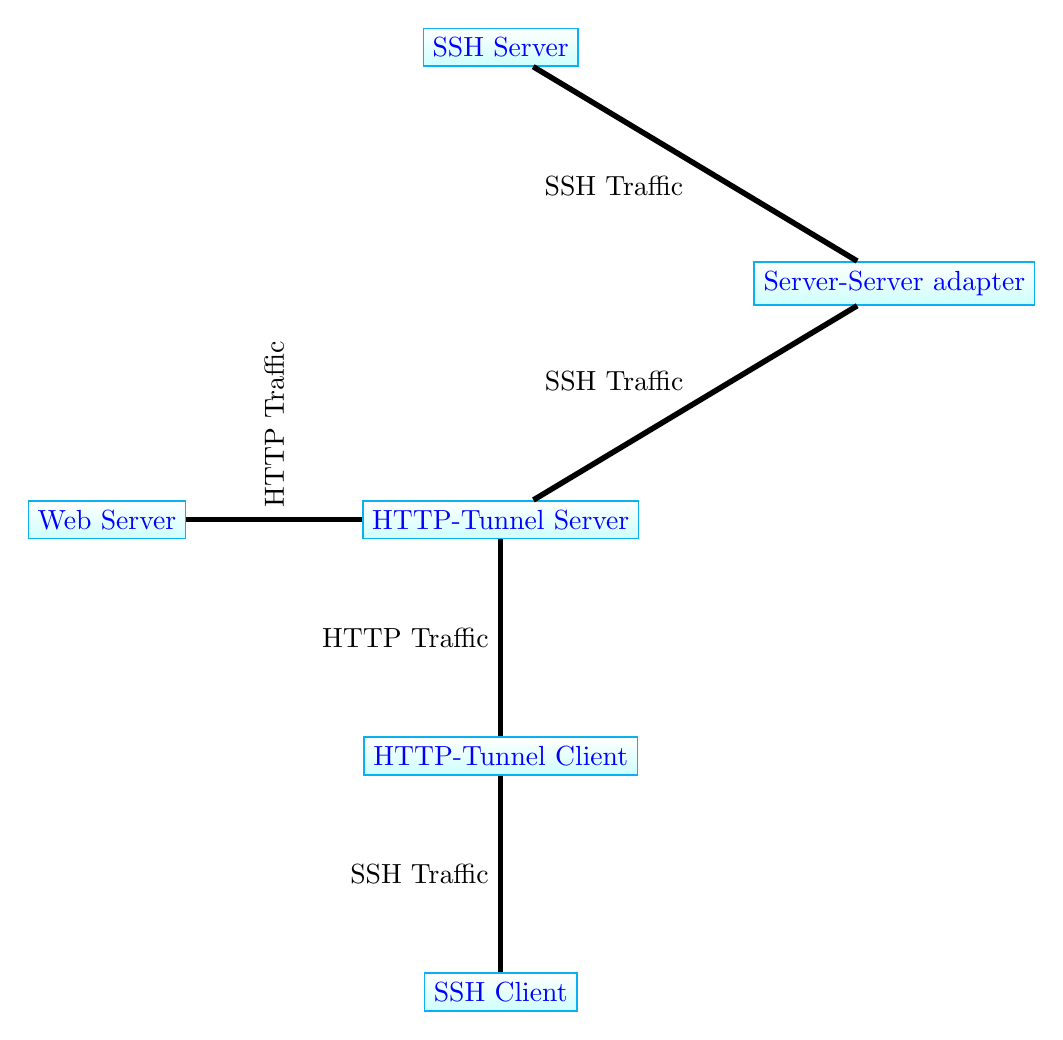
\begin{tikzpicture}[-latex ,auto ,node distance =3 cm and 5cm ,on grid, 
    semithick, state/.style={top color=white, bottom color = processblue!20, draw,processblue, text=blue, minimum width=1 cm}, line/.style={color=black,arrows=-,line cap=butt,line width=0.07cm}]
\node[state] (A)[]{HTTP-Tunnel Client};
\node[state] (B)[above=of A]{HTTP-Tunnel Server};
\node[state] (C)[left=of B]{Web Server};
\node[state] (D)[below=of A]{SSH Client};
\node[state] (E)[above right=of B]{Server-Server adapter};
\node[state] (F)[above left=of E]{SSH Server};
\path[line] (A) edge node[left] {HTTP Traffic} (B);
\path[line] (A) edge node[left] {SSH Traffic} (D);
\path[line] (B) edge node[above,rotate=90,anchor=west] {HTTP Traffic} (C);
\path[line] (B) edge node[] {SSH Traffic} (E);
\path[line] (E) edge node[] {SSH Traffic} (F);
\end{tikzpicture}
\end{center}

\subsection{HTTP-Tunnel Client}
The HTTP-Tunnel Client has a listening socket, where it receives data, and encodes it into HTTP Requests via the methods explained above.
If there is no data to be sent, it sends a request once a second, and if it receives data, it sends another straight away.
Therefore when no data is being transferred, the requests are infrequent, however when data is in the buffers, the request speed increases.

\subsection{HTTP-Tunnel Server}
The tunnel server has a listening socket where data is received, it also listens on port 80, which acts as a valid webserver if no data is received. It proxies the requests and sends them on to the webserver (which can be external or internal) to get a response




\end{document}
